%!TEX program = xelatex
\documentclass[11pt,a4paper]{article}
\usepackage[utf8]{inputenc}
\usepackage[T1]{fontenc}
\usepackage{authblk}
\usepackage{tikz}
\usepackage{pgfplots}
\usepackage{verbatim}
\usepackage{amsfonts}
\usepackage{amsmath}
\usepackage{amsthm}
\usepackage{indentfirst}
\usepackage{amssymb}
\setlength{\parindent}{0pt}
\usetikzlibrary{shapes,snakes}
\newcommand{\argmax}{\operatornamewithlimits{argmax}}
\newcommand{\argmin}{\operatornamewithlimits{argmin}}
\DeclareMathOperator{\col}{col}
\usepackage{booktabs}
\newtheorem{theorem}{Theorem}
\newtheorem{note}{Note}
\newtheorem{definition}{Definition}
\newtheorem{proposition}{Proposition}
\newtheorem{lemma}{Lemma}
\newtheorem{example}{Example}
\newtheorem{corollary}{Corollary}
\usepackage{graphicx}
\usepackage{geometry}
\usepackage{hyperref}
\newcommand{\code}{	exttt}
\geometry{a4paper,scale=0.8}
\title{STAT 425 Final Project}
\author[*]{Wenxiao Yang}
\affil[*]{Department of Mathematics, University of Illinois at Urbana-Champaign}
\date{2021}
\begin{document}
\maketitle

\section{Introduction}
This project aims to identify the optimal operating conditions for Company XX's bubble wrap lines in order to increase production capacity. We investigate the results of a completely randomized design experiment. There are two factors: \textit{line speed} (with three levels, $36,37,38 m/mm$), \textit{percent loading of additives} (with three levels, $0,2,4\%$). And one response: \textit{production rate} ($lbs/hr$). The experiment was replicated three times.\\
Our goal is to find the \textbf{optimal combination} of \textit{line speed} and \textit{percent load of additives} that results in the \textbf{highest production rate}.


\section{Analysis}
The goal of our regression analysis is to fit a two-way ANOVA model to determine the effects of various factors with different levels. We started with the full model, which included the effects of various factors as well as the interaction term.

\subsection{Full Model: Significance}
The full factor effects model is as follows:
$$Y_{ijk}=\mu+\alpha_i+\beta_j+(\alpha\beta)_{ij}+\varepsilon_{ijk}$$
$Y_{ijk}$: \textit{Production rate} for \textit{Line Speed} $i$, \textit{Percent Loading of Additives} $j$, \textit{replication} $k$.\\
$\alpha_i$: effect of \textit{Line Speed} $i$ on \textit{Production rate}.\\
$\beta_j$: effect of \textit{Percent Loading of Additives} $j$ on \textit{Production rate}.\\
$(\alpha\beta)_{ij}$: interaction term.\\
The error terms satisfy the usual assumption $\varepsilon_{i j k} \sim \mathcal{N}\left(0, \sigma^{2}\right)$.\\
Sum Constraints: $\sum_{i} \alpha_{i}=0, \sum_{j} \beta_{j}=0, \sum_{i}(\alpha \beta)_{i j}=\sum_{j}(\alpha \beta)_{i j}=0$.\\
$i=36,37,38.$\\
$j=0\%,2\%,4\%.$\\
$k=1,2,3$\\

We first plot the Interaction Plots (Figure 1) and then use the partial F-test of ANOVA table (Figure 2) to test the interaction term's significance.\\
We find the interaction is presented in the plot. However, the p-value (0.68293) of the F-test is higher than 0.05, we conclude that the interaction terms are not statistically significant. So, we can remove it from the model.\\
\begin{figure}[htb]
    \centering
    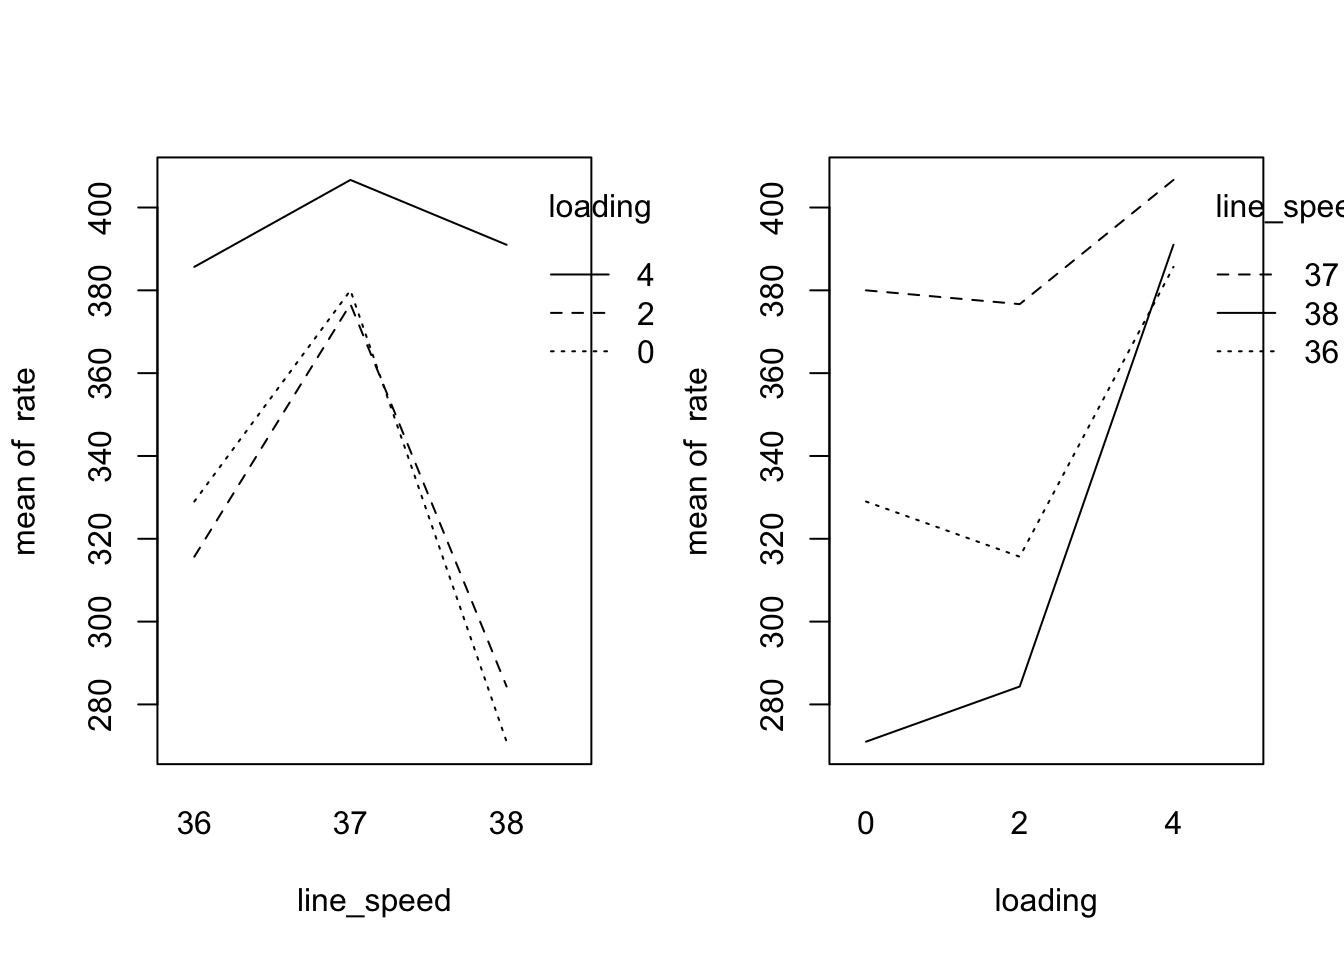
\includegraphics[scale=0.3]{inter1.png}
    \caption{Interaction Plots: Full Model}
    \label{}
\end{figure}
\begin{figure}[htb]
    \centering
    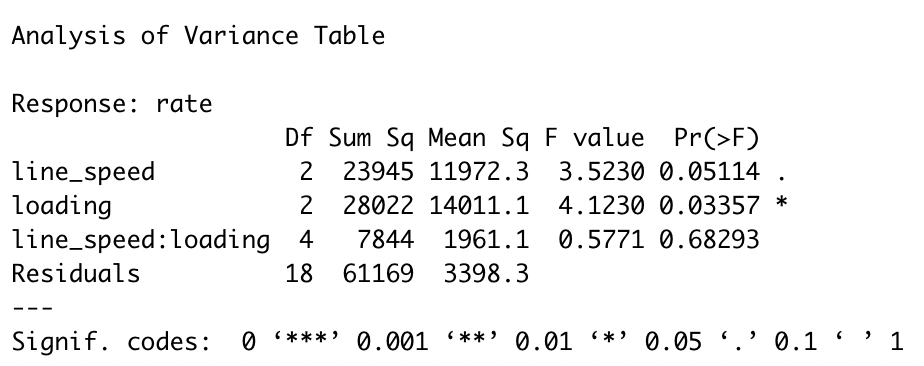
\includegraphics[scale=0.8]{inter2.png}
    \caption{ANOVA Table: Full model}
    \label{}
\end{figure}


\subsection{Additive Model: Significance}
Then we fit the regression of the additive model:
$$Y_{ijk}=\mu+\alpha_i+\beta_j+\varepsilon_{ijk}$$
$Y_{ijk}$: \textit{Production rate} for \textit{Line Speed} $i$, \textit{Percent Loading of Additives} $j$, \textit{replication} $k$.\\
$\alpha_i$: effect of \textit{Line Speed} $i$ on \textit{Production rate}.\\
$\beta_j$: effect of \textit{Percent Loading of Additives} $j$ on \textit{Production rate}.\\
The error terms satisfy the usual assumption $\varepsilon_{i j k} \sim \mathcal{N}\left(0, \sigma^{2}\right)$.\\
Sum Constraints: $\sum_{i} \alpha_{i}=0, \sum_{j} \beta_{j}=0$.\\
$i=36,37,38.$\\
$j=0\%,2\%,4\%.$\\
$k=1,2,3$\\

We use the partial F-test of the ANOVA table (Figure 3) to test the significance of both factors. Since the p-values of both factors are lower than 0.05 (\textit{Line Speed}: 0.03777, \textit{Percent Loading of Additives}: 0.02355), we can conclude that both factors are statistically significant.
\begin{figure}[htb]
    \centering
    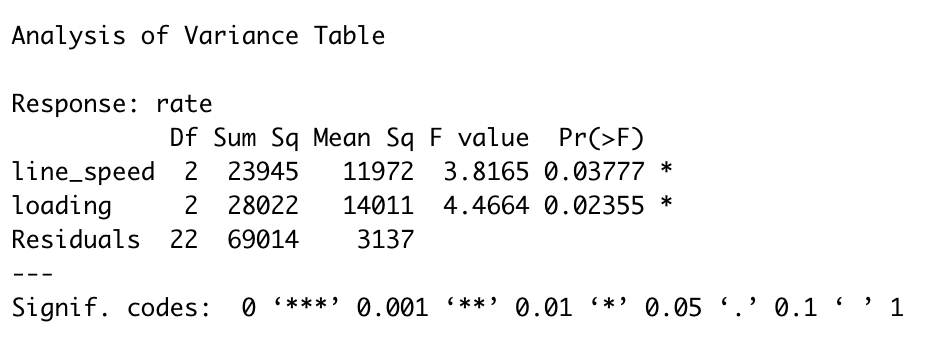
\includegraphics[scale=0.8]{add1.png}
    \caption{ANOVA Table: Additive Model}
    \label{}
\end{figure}

\subsection{Additive Model: Check Assumptions}
Then we need to check the assumptions of the additive model.\\
To validate the assumptions, we perform the studentized Breusch-Pagan test (Figure 4), the Kolmogorov-Smirnov test (Figure 5), and the diagnostic plots (Figure 6) which include the 1. Residuals vs. Fitted plot and the 2. Normal Q-Q plot.\\
1. \textbf{Constancy of Variance (Homoscedasticity)}: By the Residuals vs. Fitted plot and studentized Breusch-Pagan test result ($p-value=0.117>0.05$), we can conclude homoscedasticity assumption holds in the additive model.\\
2. \textbf{Normality}: By the Q-Q plot (obviously not a line) and Kolmogorov-Smirnov test result ($p-value=1.156e-07$), we can conclude Normality doesn't hold in the additive model.
\begin{figure}[htb]
    \centering
    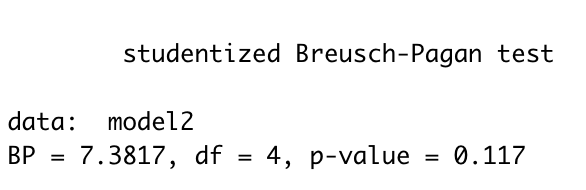
\includegraphics[scale=1]{BP1}
    \caption{Studentized Breusch-Pagan Test Result: Additive Model}
    \label{}
\end{figure}
\begin{figure}[htb]
    \centering
    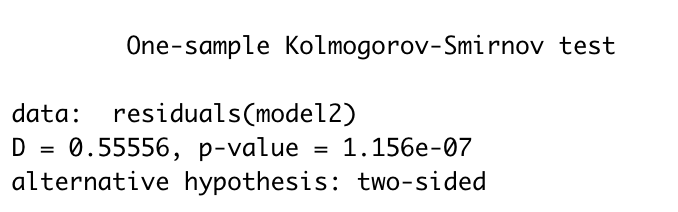
\includegraphics[scale=1]{KS1}
    \caption{Kolmogorov-Smirnov Test Result: Additive Model}
    \label{}
\end{figure}
\begin{figure}[htb]
    \centering
    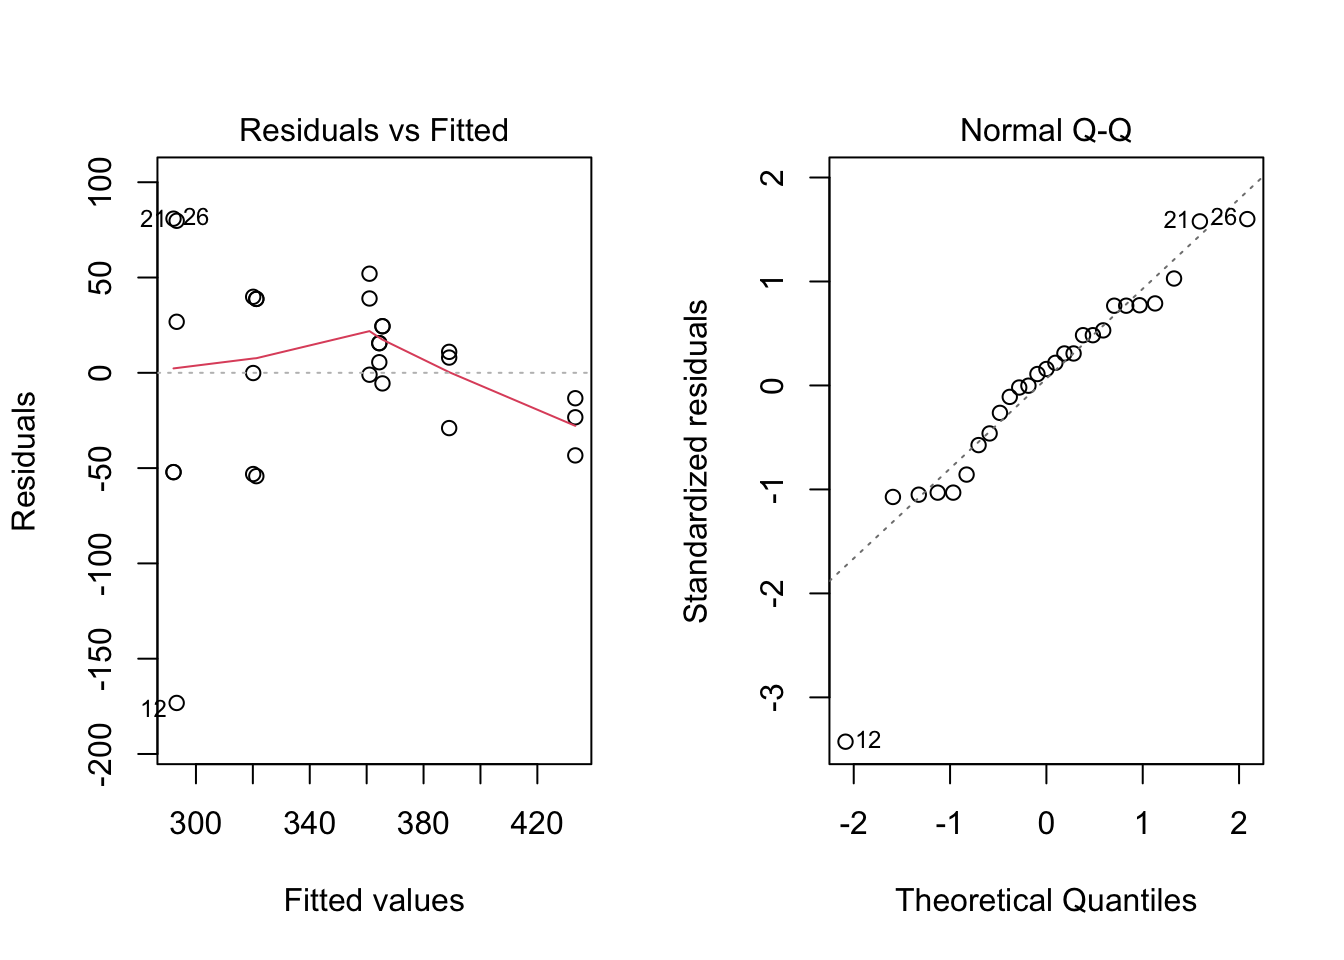
\includegraphics[scale=0.3]{DP1}
    \caption{Diagnostic Plots: Additive Model}
    \label{}
\end{figure}

\subsection{Box-cox Transformation}
In the additive model, the normality assumption is violated. Because our response variable only contains positive values, the Box-cox transformation may be used to address assumptions violations. The $\lambda$ found by Box-cox transformation is $5.151515$ (Figure 7). We use $\lambda=5.5$ to transform the model. Then the new transformed model is as following:
$$\frac{Y_{ijk}^{5.5}-1}{5.5}=\mu+\alpha_i+\beta_j+(\alpha\beta)_{ij}+\varepsilon_{ijk}$$
$Y_{ijk}$: \textit{Production rate} for \textit{Line Speed} $i$, \textit{Percent Loading of Additives} $j$, \textit{replication} $k$.\\
$\alpha_i$: effect of \textit{Line Speed} $i$ on \textit{Production rate}.\\
$\beta_j$: effect of \textit{Percent Loading of Additives} $j$ on \textit{Production rate}.\\
$(\alpha\beta)_{ij}$: interaction term.\\
The error terms satisfy the usual assumption $\varepsilon_{i j k} \sim \mathcal{N}\left(0, \sigma^{2}\right)$.\\
Sum Constraints: $\sum_{i} \alpha_{i}=0, \sum_{j} \beta_{j}=0, \sum_{i}(\alpha \beta)_{i j}=\sum_{j}(\alpha \beta)_{i j}=0$.\\
$i=36,37,38.$\\
$j=0\%,2\%,4\%.$\\
$k=1,2,3$
\begin{figure}[htb]
    \centering
    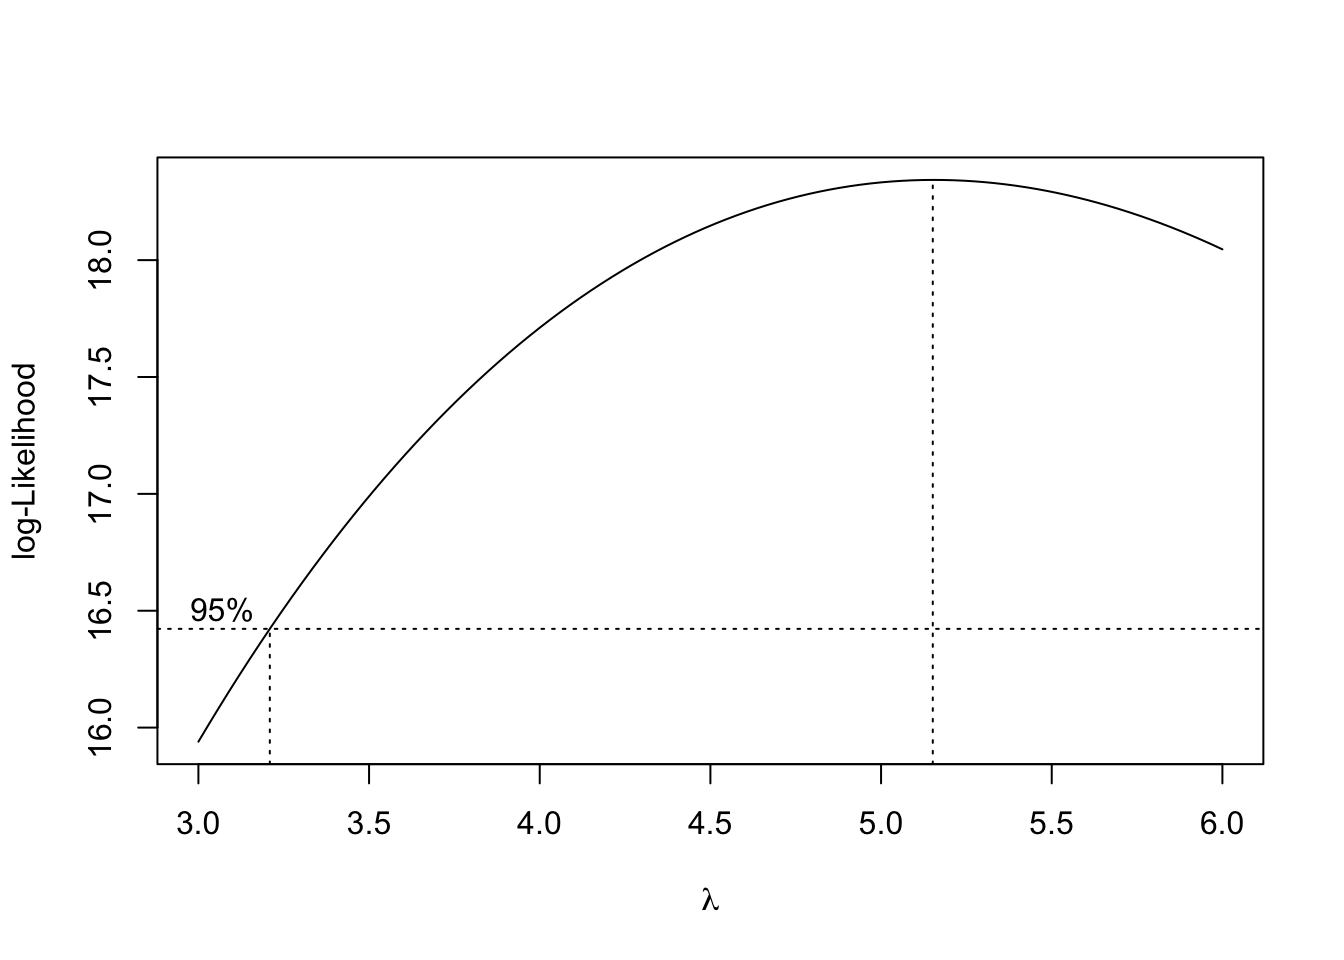
\includegraphics[scale=0.3]{lam.png}
    \caption{Box-cox Transformation: Find Optimal $\lambda$}
    \label{}
\end{figure}


\subsection{New Transformed Model: Significance}
For the new transformed model, we also need to check whether the interaction is significant or not. We plot the Interaction Plots (Figure 8) and then use the partial F-test of ANOVA table (Figure 9) to test the interaction term's significance.\\
We find the interaction is presented in the plot. However, the p-value (0.9063497) of the F-test is higher than 0.05, we conclude that the interaction terms are not statistically significant. So, we can remove it from the model.\\
\begin{figure}[htb]
    \centering
    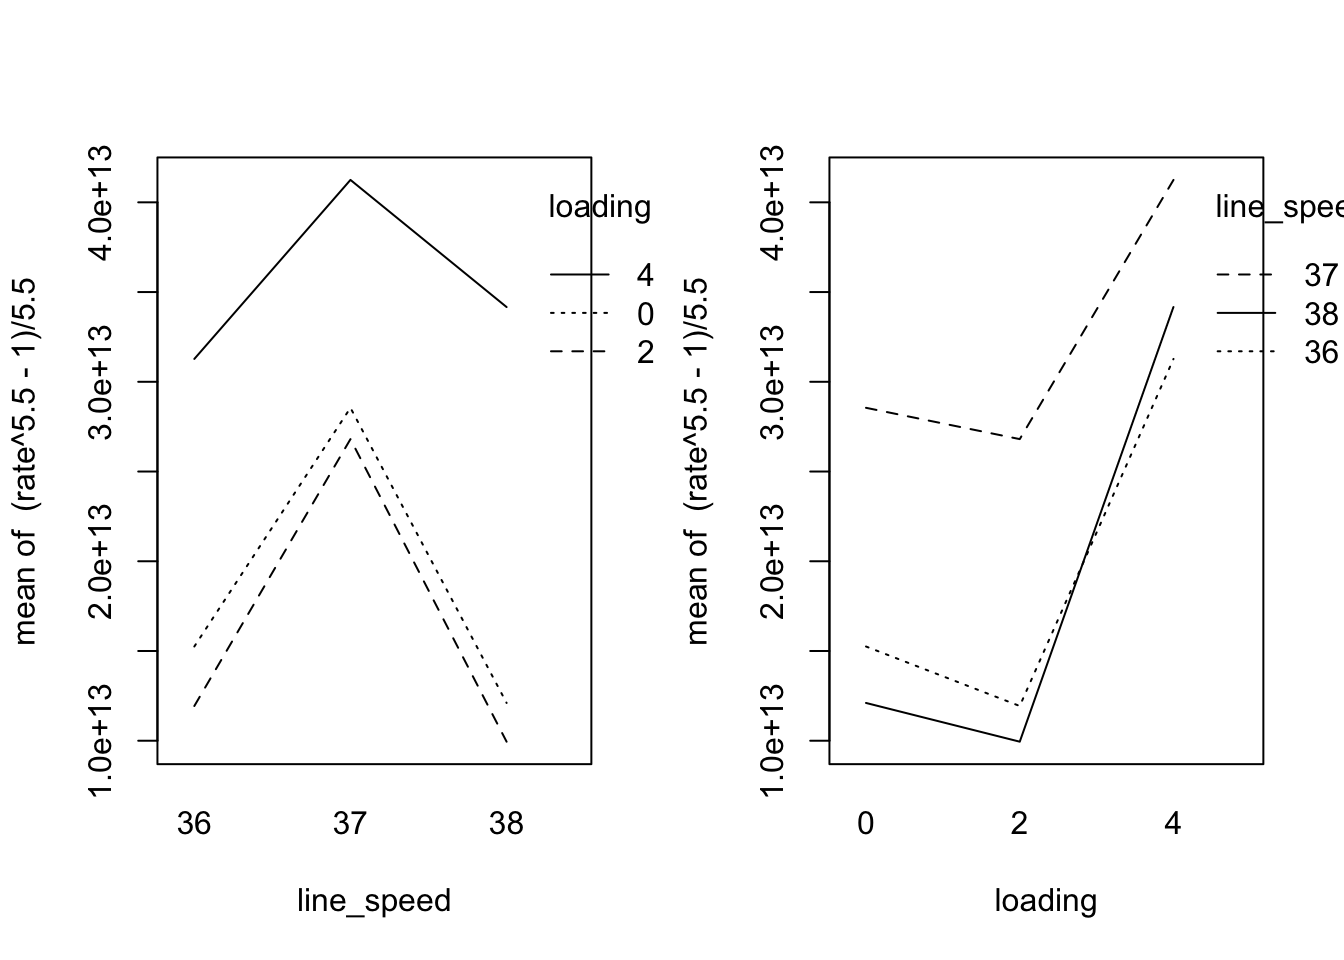
\includegraphics[scale=0.3]{inter3.png}
    \caption{Interaction Plots: New Transformed Model}
    \label{}
\end{figure}
\begin{figure}[htb]
    \centering
    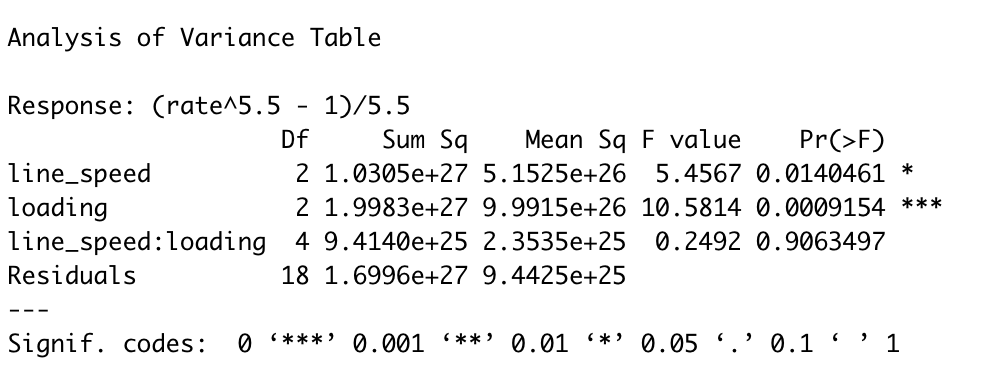
\includegraphics[scale=0.8]{inter4.png}
    \caption{ANOVA Table: New Transformed Model}
    \label{}
\end{figure}

\subsection{New Additive Model: Significance}
Then we fit the regression of the additive model:
$$\frac{Y_{ijk}^{5.5}-1}{5.5}=\mu+\alpha_i+\beta_j+\varepsilon_{ijk}$$
$Y_{ijk}$: \textit{Production rate} for \textit{Line Speed} $i$, \textit{Percent Loading of Additives} $j$, \textit{replication} $k$.\\
$\alpha_i$: effect of \textit{Line Speed} $i$ on \textit{Production rate}.\\
$\beta_j$: effect of \textit{Percent Loading of Additives} $j$ on \textit{Production rate}.\\
The error terms satisfy the usual assumption $\varepsilon_{i j k} \sim \mathcal{N}\left(0, \sigma^{2}\right)$.\\
Sum Constraints: $\sum_{i} \alpha_{i}=0, \sum_{j} \beta_{j}=0$.\\
$i=36,37,38.$\\
$j=0\%,2\%,4\%.$\\
$k=1,2,3$\\

We use the partial F-test of the ANOVA table (Figure 10) to test the significance of both factors. Since the p-values of both factors are lower than 0.05 (\textit{Line Speed}: 0.0067840, \textit{Percent Loading of Additives}: 0.0002654), we can conclude that both factors are statistically significant.
\begin{figure}[htb]
    \centering
    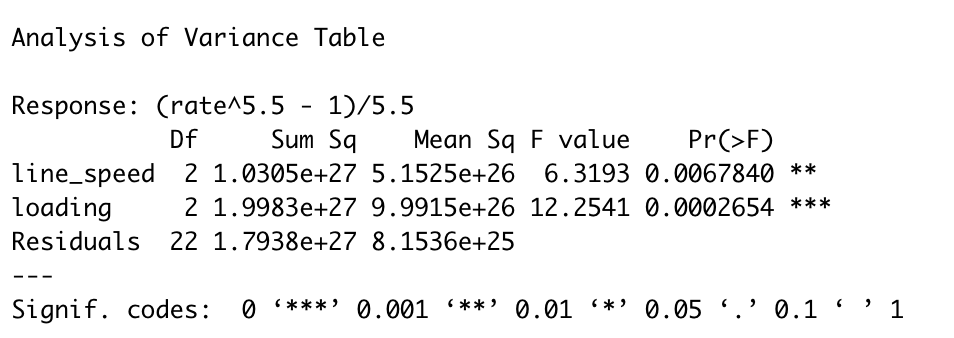
\includegraphics[scale=0.8]{add2.png}
    \caption{ANOVA Table: New Additive Model}
    \label{}
\end{figure}


\subsection{New Additive Model: Check Assumptions}
Then we need to check the assumptions of the new additive model.\\
To validate the assumptions, we perform the studentized Breusch-Pagan test (Figure 11), the Kolmogorov-Smirnov test (Figure 12), and the diagnostic plots (Figure 13) which include the 1. Residuals vs. Fitted plot and the 2. Normal Q-Q plot.\\
1. \textbf{Constancy of Variance (Homoscedasticity)}: By the Residuals vs. Fitted plot and studentized Breusch-Pagan test result ($p-value=0.117>0.05$), we can conclude homoscedasticity assumption holds in the additive model.\\
2. \textbf{Normality}: By the Q-Q plot (obviously not a line) and Kolmogorov-Smirnov test result ($p-value=1.156e-07$), we can conclude Normality doesn't hold in the additive model.
\begin{figure}[htb]
    \centering
    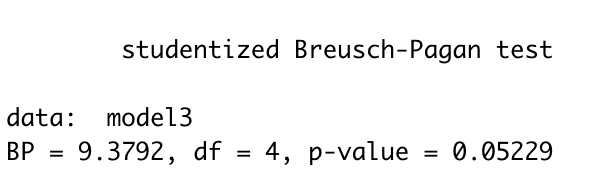
\includegraphics[scale=1]{BP2}
    \caption{Studentized Breusch-Pagan Test Result: New Additive Model}
    \label{}
\end{figure}
\begin{figure}[htb]
    \centering
    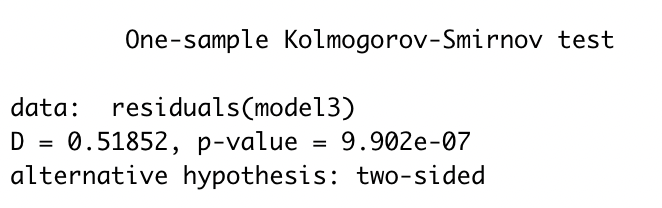
\includegraphics[scale=1]{KS2}
    \caption{Kolmogorov-Smirnov Test Result: New Additive Model}
    \label{}
\end{figure}
\begin{figure}[htb]
    \centering
    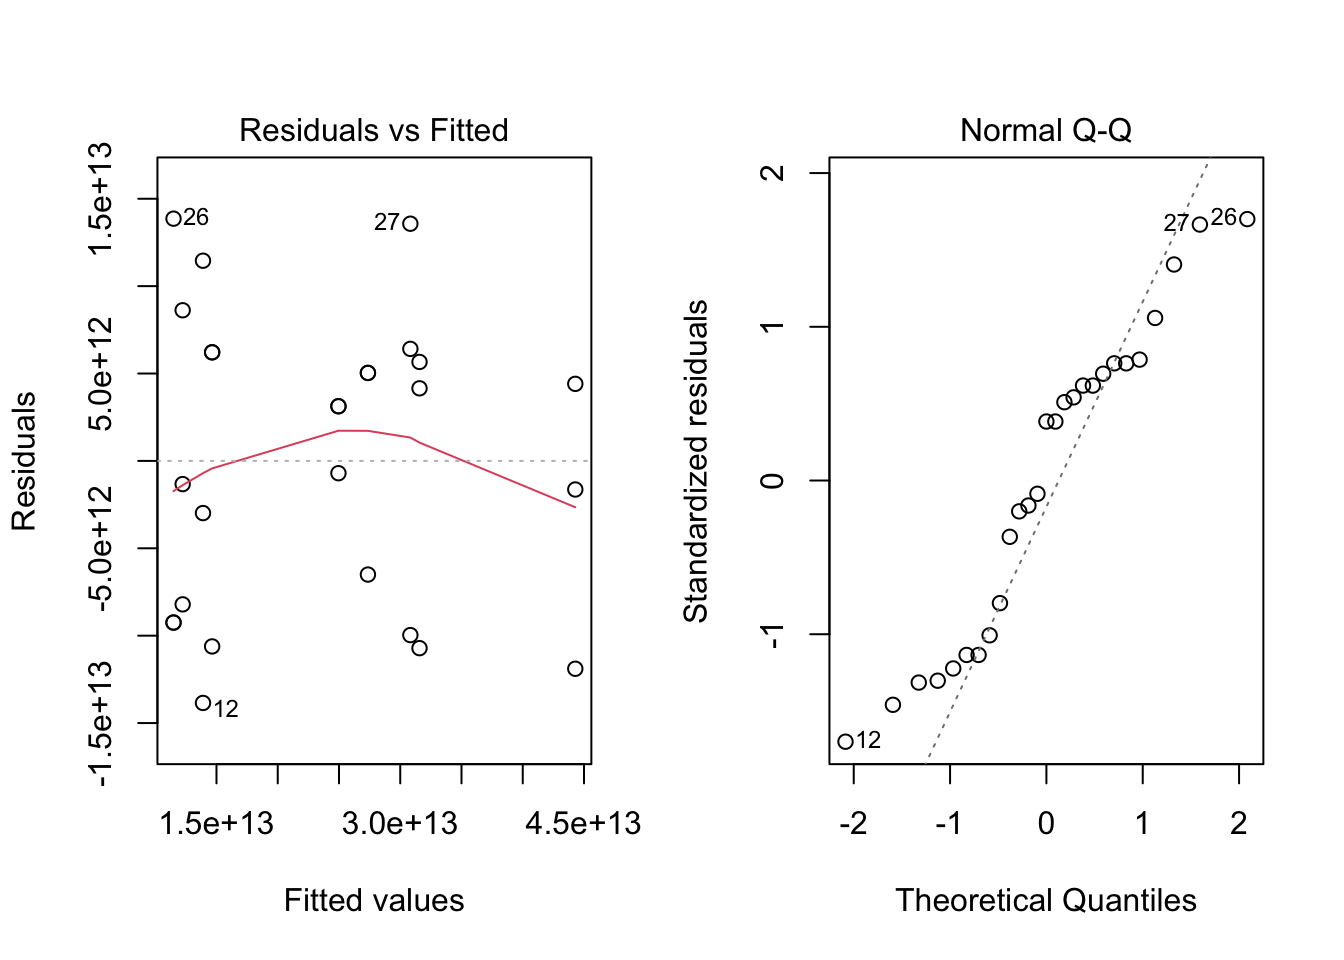
\includegraphics[scale=0.3]{DP2}
    \caption{Diagnostic Plots: New Additive Model}
    \label{}
\end{figure}

The Box-cox transformation is incapable of resolving the normality violation issue. The new additive model, on the other hand, has a higher Adjusted R-squared (Adjusted $R^2=0.5604$, Figure 14) than the previous additive model (Adjusted $R^2=0.3258$, Figure 15). As a result, we should draw conclusions using the new additive model.
\begin{figure}[htb]
    \centering
    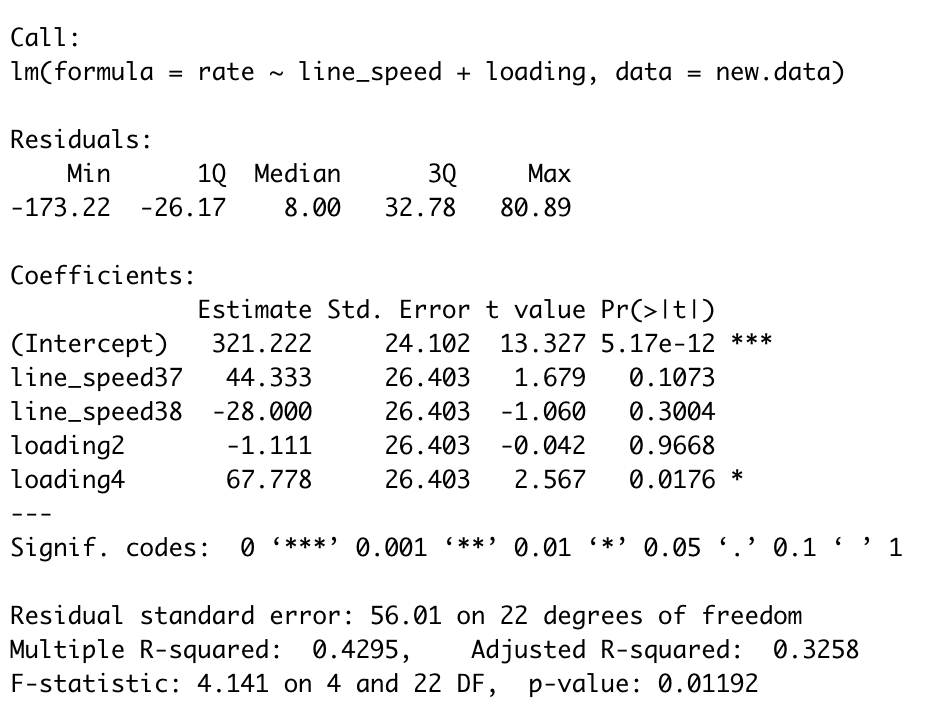
\includegraphics[scale=0.8]{R1}
    \caption{Regression Summary: Additive Model}
    \label{}
\end{figure}
\begin{figure}[htb]
    \centering
    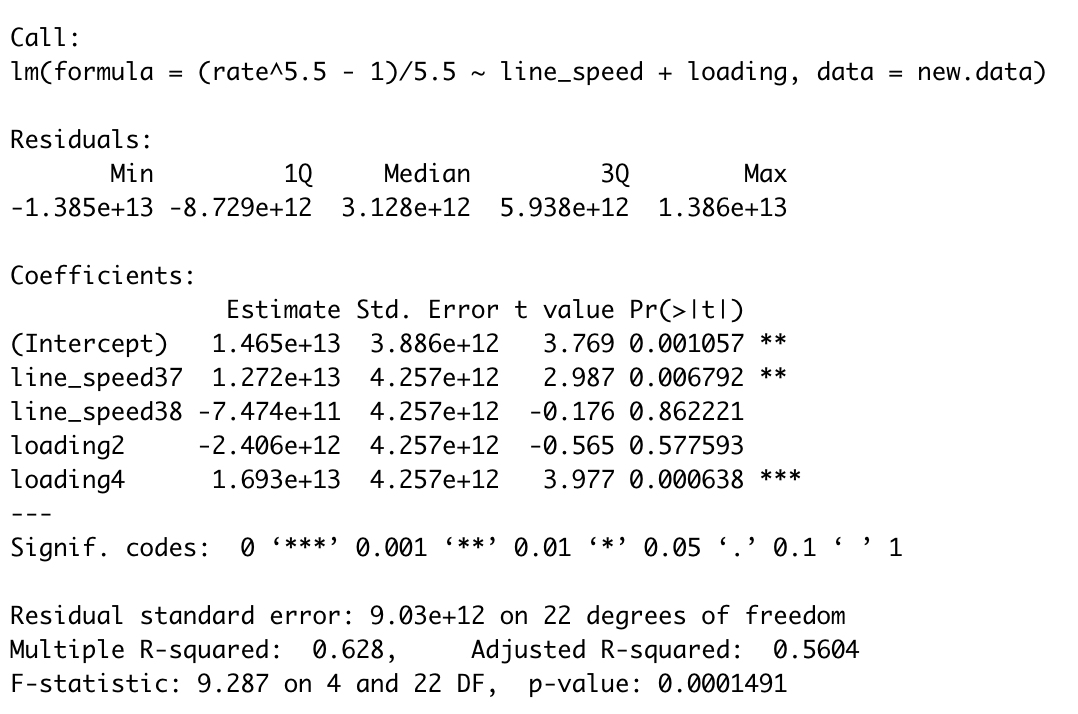
\includegraphics[scale=0.8]{R2}
    \caption{Regression Summary: New Additive Model}
    \label{}
\end{figure}

\subsection{Tukey’s Paired Comparison}
Then we can use Tukey’s paired comparison to test the difference between different factor levels.\\
1. \textbf{Line Speed}: According to the Tukey’s paired comparison results (Figure16, Figure 17), the 95\% family-wise confidence level of \textit{Effect of 37 Line Speed} - \textit{Effect of 36 Line Speed} is $[2.022656e+12,2.340860e+13]$; \textit{Effect of 38 Line Speed} - \textit{Effect of 36 Line Speed} is $[-1.144041e+13 ,9.945539e+12]$; \textit{Effect of 38 Line Speed} - \textit{Effect of 37 Line Speed} is $[-2.415603e+13, -2.770089e+12]$. Then we can conclude \textit{Effect of 37 Line Speed}$>${Effect of 38 Line Speed}$\approx$\textit{Effect of 36 Line Speed}, \textbf{37 is the best factor level of line speed}.\\
2. \textbf{Percent Loading of Additives}: According to the Tukey’s paired comparison results (Figure18, Figure 19), the 95\% family-wise confidence level of \textit{Effect of 2\% Percent Loading of Additives} - \textit{Effect of 0\% Percent Loading of Additives} is $[-1.309924e+13, 8.286709e+12]$; \textit{Effect of 4\% Percent Loading of Additives} - \textit{Effect of 0\% Percent Loading of Additives} is $[6.234150e+12 2.762009e+13]$; \textit{Effect of 4\% Percent Loading of Additives} - \textit{Effect of 2\% Percent Loading of Additives} is $[8.640413e+12 3.002636e+13]$. Then we can conclude \textit{Effect of 4\% Percent Loading of Additives}$>${Effect of 2\% Percent Loading of Additives}$\approx$\textit{Effect of 0\% Percent Loading of Additives}, \textbf{4\% is the best factor level of percent loading of additives}.\\
\begin{figure}[htb]
    \centering
    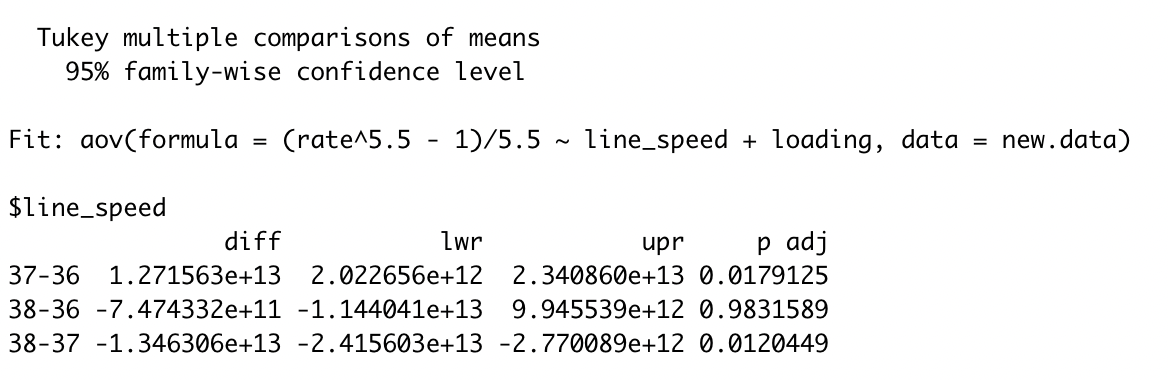
\includegraphics[scale=0.8]{CI1}
    \caption{Confidence Interval: Line Speed}
    \label{}
\end{figure}
\begin{figure}[htb]
    \centering
    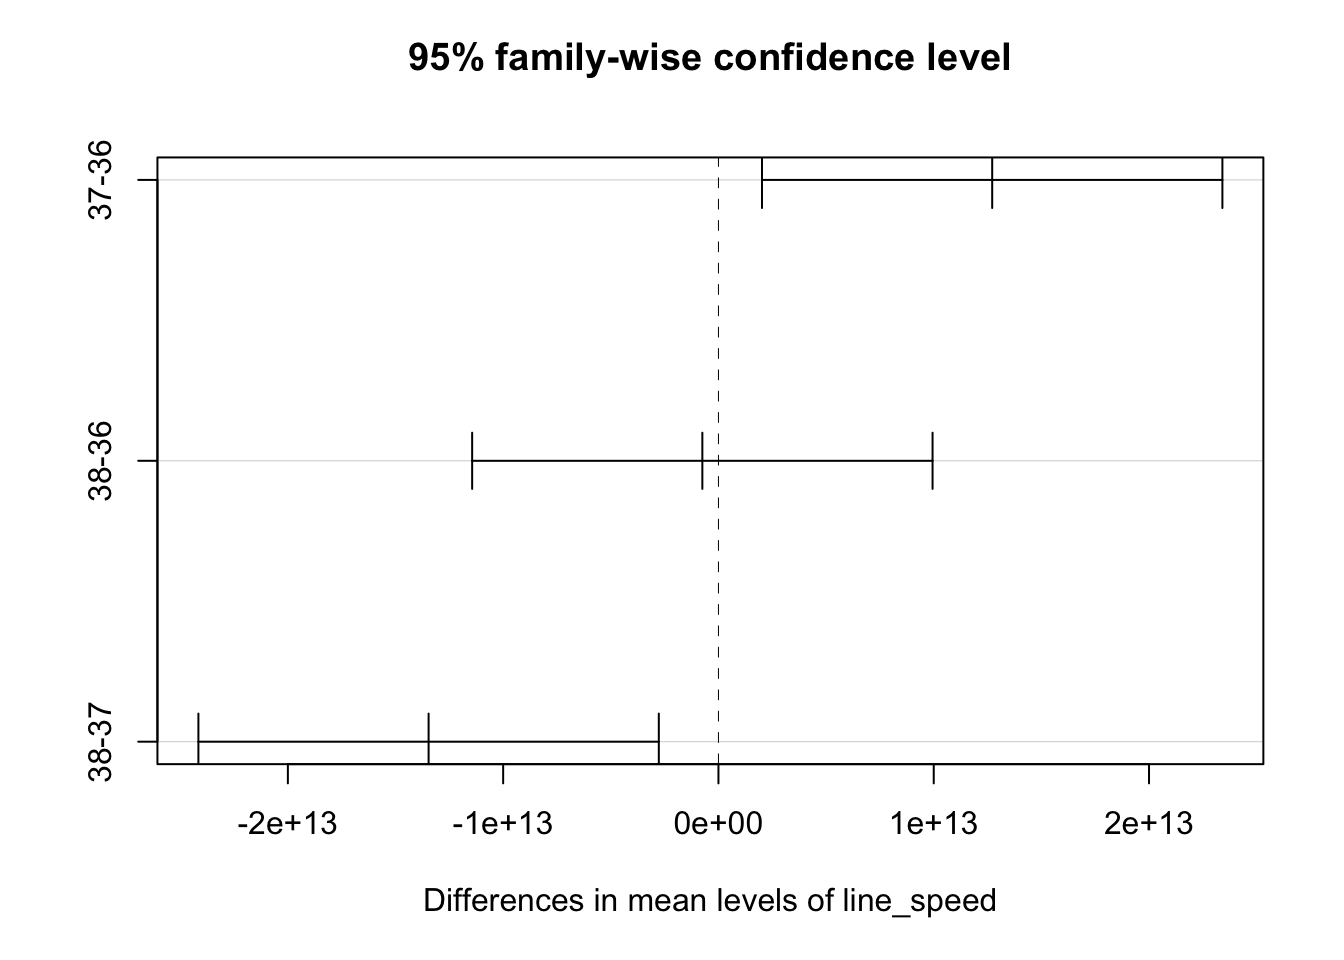
\includegraphics[scale=0.3]{CIP1}
    \caption{Confidence Interval Plot: Line Speed}
    \label{}
\end{figure}
\begin{figure}[htb]
    \centering
    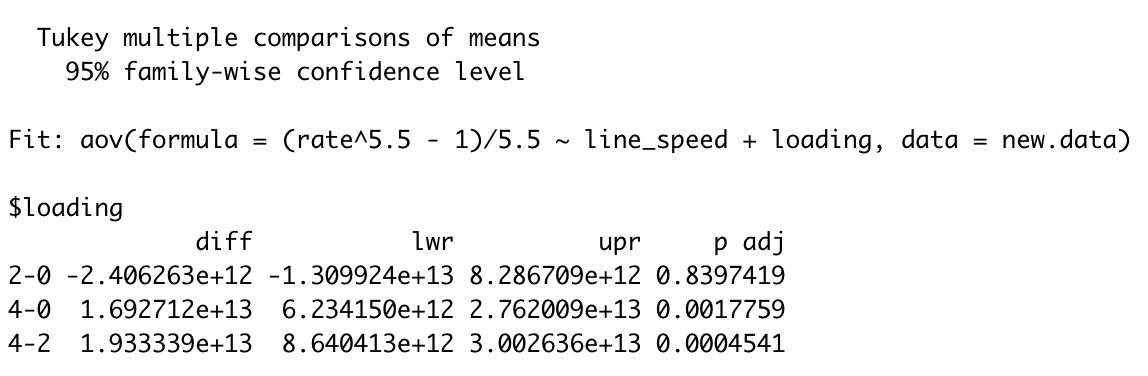
\includegraphics[scale=0.8]{CI2}
    \caption{Confidence Interval: Percent Loading of Additives}
    \label{}
\end{figure}
\begin{figure}[htb]
    \centering
    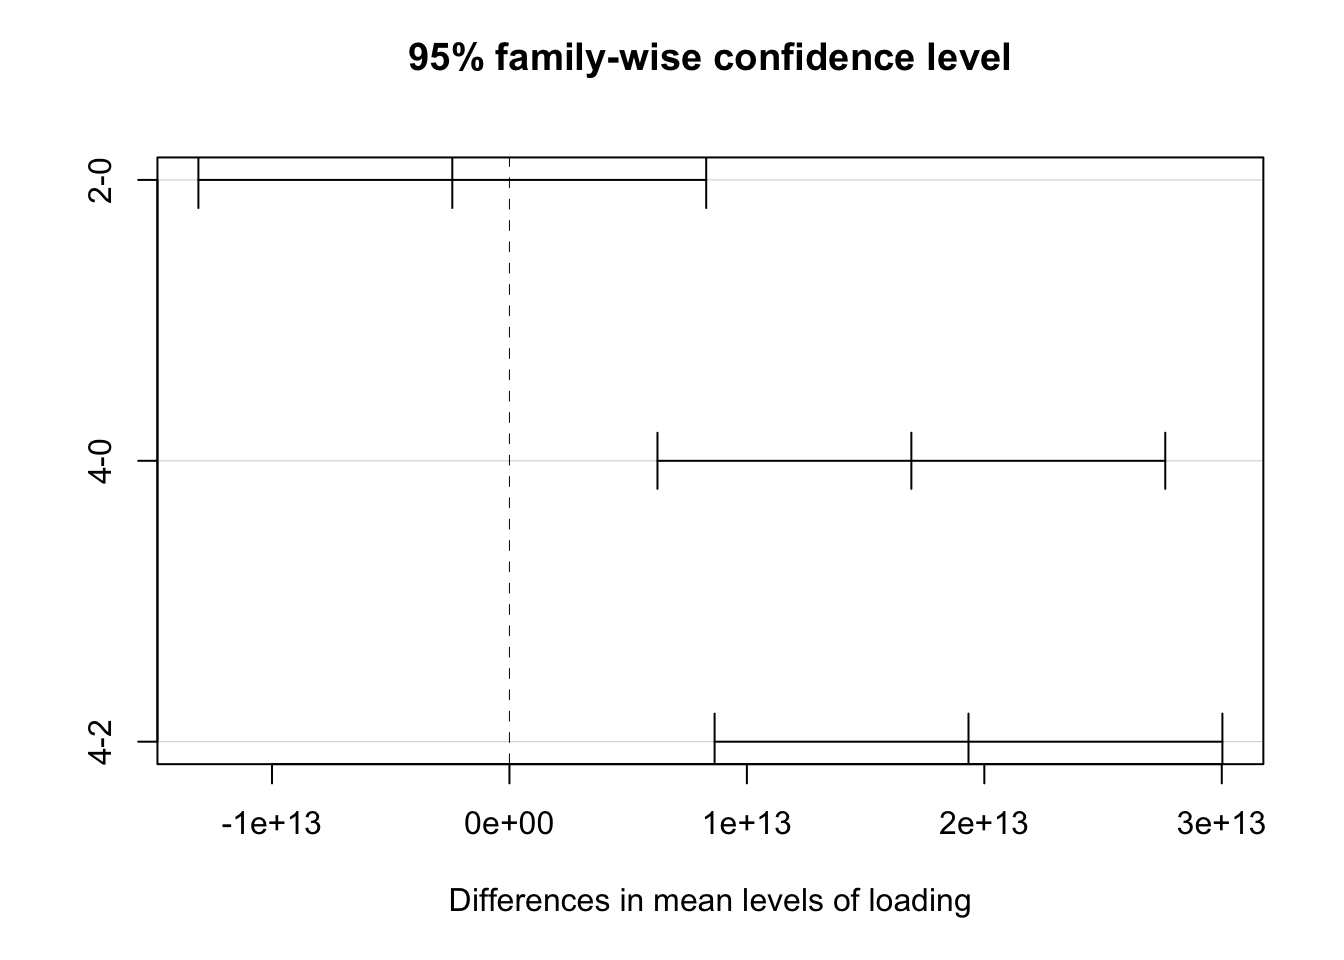
\includegraphics[scale=0.3]{CIP2}
    \caption{Confidence Interval Plot: Percent Loading of Additives}
    \label{}
\end{figure}

































\end{document}